\documentclass{article}

\usepackage{graphicx}
\usepackage{tikz}
\usepackage{tikzsymbols}
\usetikzlibrary{calc,patterns,shapes.geometric}
\pagestyle{empty}
\usepackage[margin=0pt]{geometry}
\geometry{papersize={14in,12in}}

\def\centerarc[#1](#2)(#3:#4:#5){\draw[#1] ($(#2)+({#5*cos(#3)},{#5*sin(#3)})$) arc (#3:#4:#5);}

\begin{document}
	\begin{figure}
		\centering
		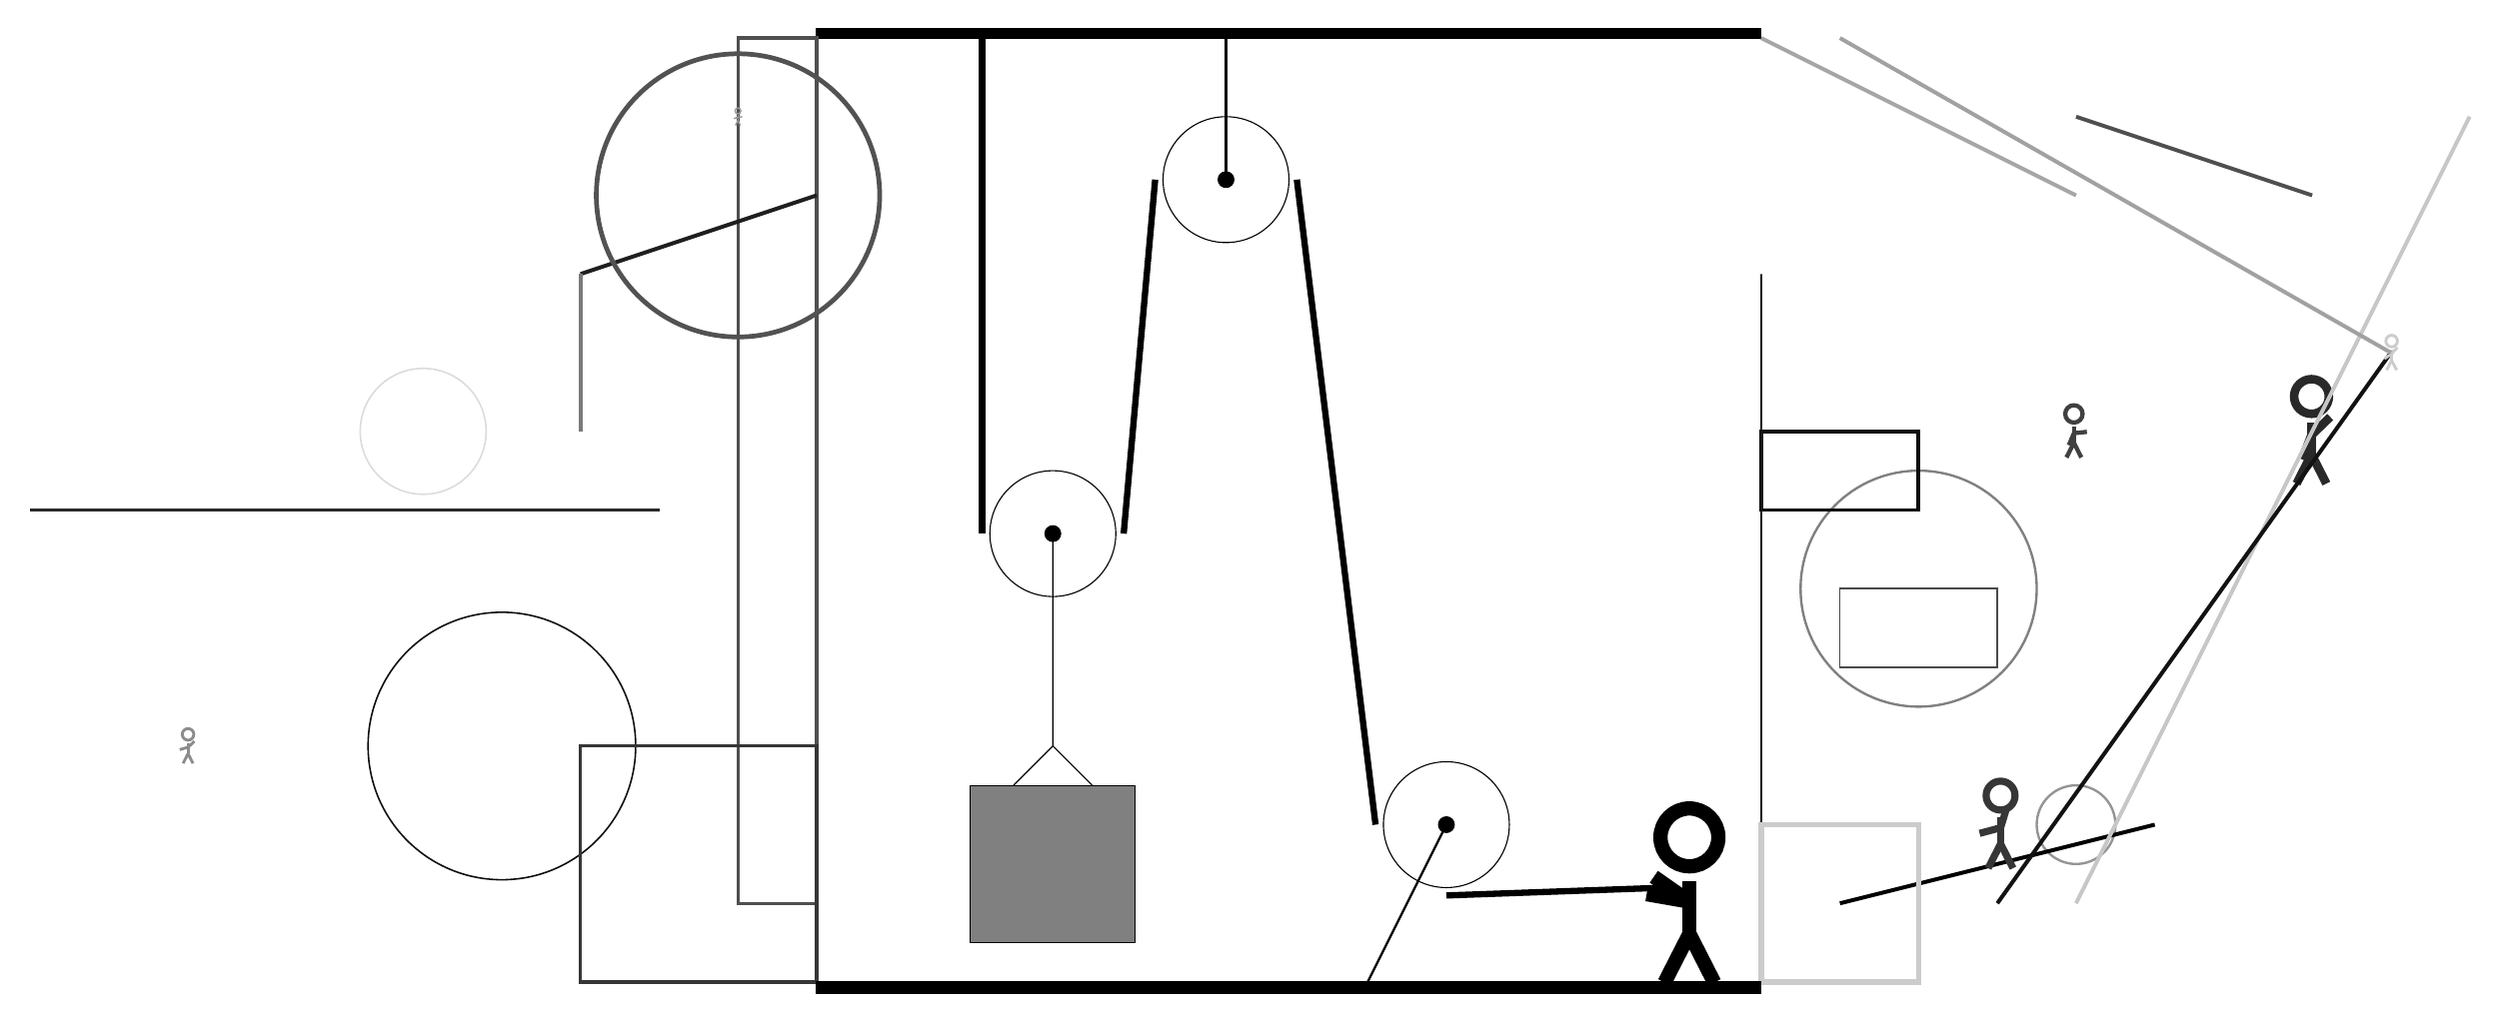
\begin{tikzpicture}
			%%%%% START %%%%%
			
			\draw[fill=black] (-2, 9) rectangle (10, 9.125);
			
			\draw (3.2, 7.2) circle (0.8);
			\draw[fill=black] (3.2, 7.2) circle (0.1);
			\draw[thick] (3.2, 7.2) -- (3.2, 9);
			
			\draw (6, -1) circle (0.8);
			\draw[fill=black] (6, -1) circle (0.1);
			\draw[thick] (6, -1) -- (5, -3);
			
			\draw [line width=0.3mm, color=black!50](12, 2) circle (1.5);
			
			\draw[line width=0.4mm, color=black!69] (-2, -2) rectangle (-3, 9);
			\node[line width=0.7mm, color=black!84] at (17, 4) {\Strichmaxerl[6][69][44]};
			\draw [line width=0.2mm, color=black!14](-7, 4) circle (0.8);
			\draw [line width=0.3mm, color=black!42](14, -1) circle (0.5);
			
			\node[line width=0.4mm, color=black!40] at (-3, 8) {\Strichmaxerl[1][16][7]};
			\draw[line width=0.5mm, color=black!88](-2, 7) -- (-5, 6);
			
			\draw[line width=0.5mm, color=black!100](11, -2) -- (15, -1);
			\draw[line width=0.2mm, color=black!71] (11, 1) rectangle (13, 2);
			\draw [line width=0.2mm, color=black!95](-6, 0) circle (1.7);
			\draw[line width=0.5mm, color=black!95] (10, 3) rectangle (12, 4);
			
			\draw[line width=0.4mm, color=black!79] (-2, -3) rectangle (-5, 0);
			\draw[line width=0.5mm, color=black!22](14, -2) -- (19, 8);
			
			\draw [line width=0.6mm, color=black!68](-3, 7) circle (1.8);
			\draw[line width=0.5mm, color=black!93](13, -2) -- (18, 5);
			\draw[line width=0.3mm, color=black!91] (10, -3) rectangle (10, 6);
			\node[line width=0.3mm, color=black!45] at (-10, 0) {\Strichmaxerl[2][16][43]};
			\draw[line width=0.5mm, color=black!84](-4, 3) -- (-12, 3);
			\draw[line width=0.5mm, color=black!35](14, 7) -- (10, 9);
			
			\node[line width=0.5mm, color=black!20] at (18, 5) {\Strichmaxerl[2][33][49]};
			\draw[line width=0.5mm, color=black!52](-5, 6) -- (-5, 4);
			\node[line width=0.2mm, color=black!79] at (13, -1) {\Strichmaxerl[5][15][73]};
			\draw[line width=0.7mm, color=black!20] (10, -3) rectangle (12, -1);
			\node[line width=0.7mm, color=black!75] at (14, 4) {\Strichmaxerl[3][67][6]};
			\draw[line width=0.5mm, color=black!37](11, 9) -- (18, 5);
			\draw[line width=0.5mm, color=black!69](14, 8) -- (17, 7);
			
			\draw (1, 2.7) circle (0.8);
			\draw[fill=black] (1, 2.7) circle (0.1);
			
			\draw (1, 2.7) -- (1, 0) -- (0.5, -0.5);
			\draw (1, 0) -- (1.5, -0.5);
			\draw[fill=black!50] (-0.05, -0.5) rectangle (2.05, -2.5);
			
			\draw[line width=0.8mm] (0.1, 9) -- (0.1, 2.7);
			\centerarc[line width=0.8mm](1, 2.7)(180:360:0.9);
			\draw[line width=0.8mm](1.9, 2.7) -- (2.3, 7.2);
			\centerarc[line width=0.8mm](3.2, 7.2)(0:180:0.9);
			\draw[line width=0.8mm](4.1, 7.2) -- (5.1, -1);
			\centerarc[line width=0.8mm](6, -1)(180:270:0.9);
			\draw[line width=0.8mm](6, -1.9) -- (8.8, -1.8);
			
			\node at (9, -1.9) {\Strichmaxerl[10][-35][170]};
			
			\draw[fill=black] (-2, -3) rectangle (10, -3.15);
			
			%%%%% END %%%%%
		\end{tikzpicture}
	\end{figure}	
\end{document}